%********************************************************************
% Appendix
%*******************************************************
% If problems with the headers: get headings in appendix etc. right
%\markboth{\spacedlowsmallcaps{Appendix}}{\spacedlowsmallcaps{Appendix}}
\chapter{Appendix}

%\section{Quenching resistor}



\section{Breakdown Voltage}
Breakdown voltages fit used for $V_{bd}$ channel comparison with the VATA64 method and the waveform \& PDE analysis. 
\begin{figure}[htbp]
  \centering
  \begin{subfigure}{0.48\textwidth}
    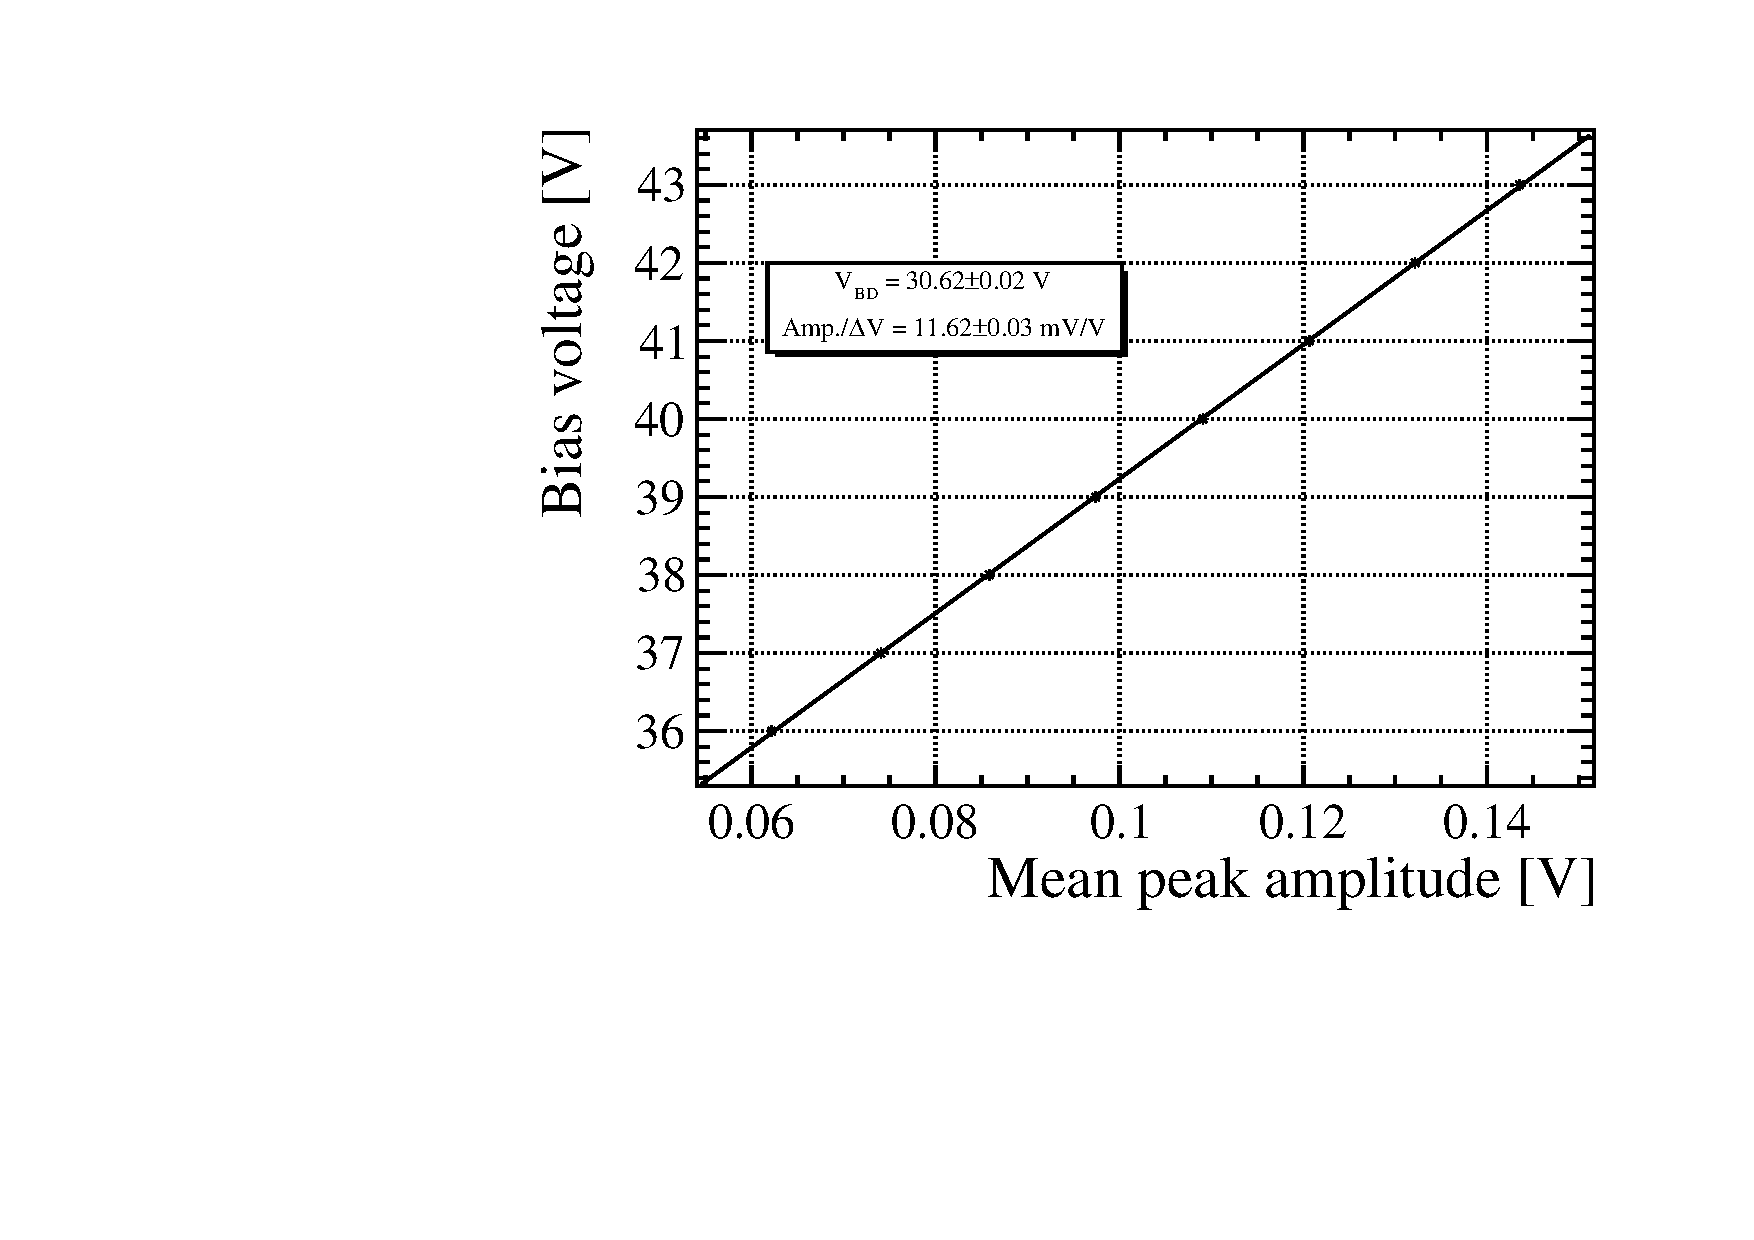
\includegraphics[width=1\linewidth]{gfx/plots/WA/16/Breakdown_voltage70.pdf}
    \caption{\SI{16}{\micro m} channel $70$.}  
  \end{subfigure}
  \hfill
  \begin{subfigure}{0.48\textwidth}
    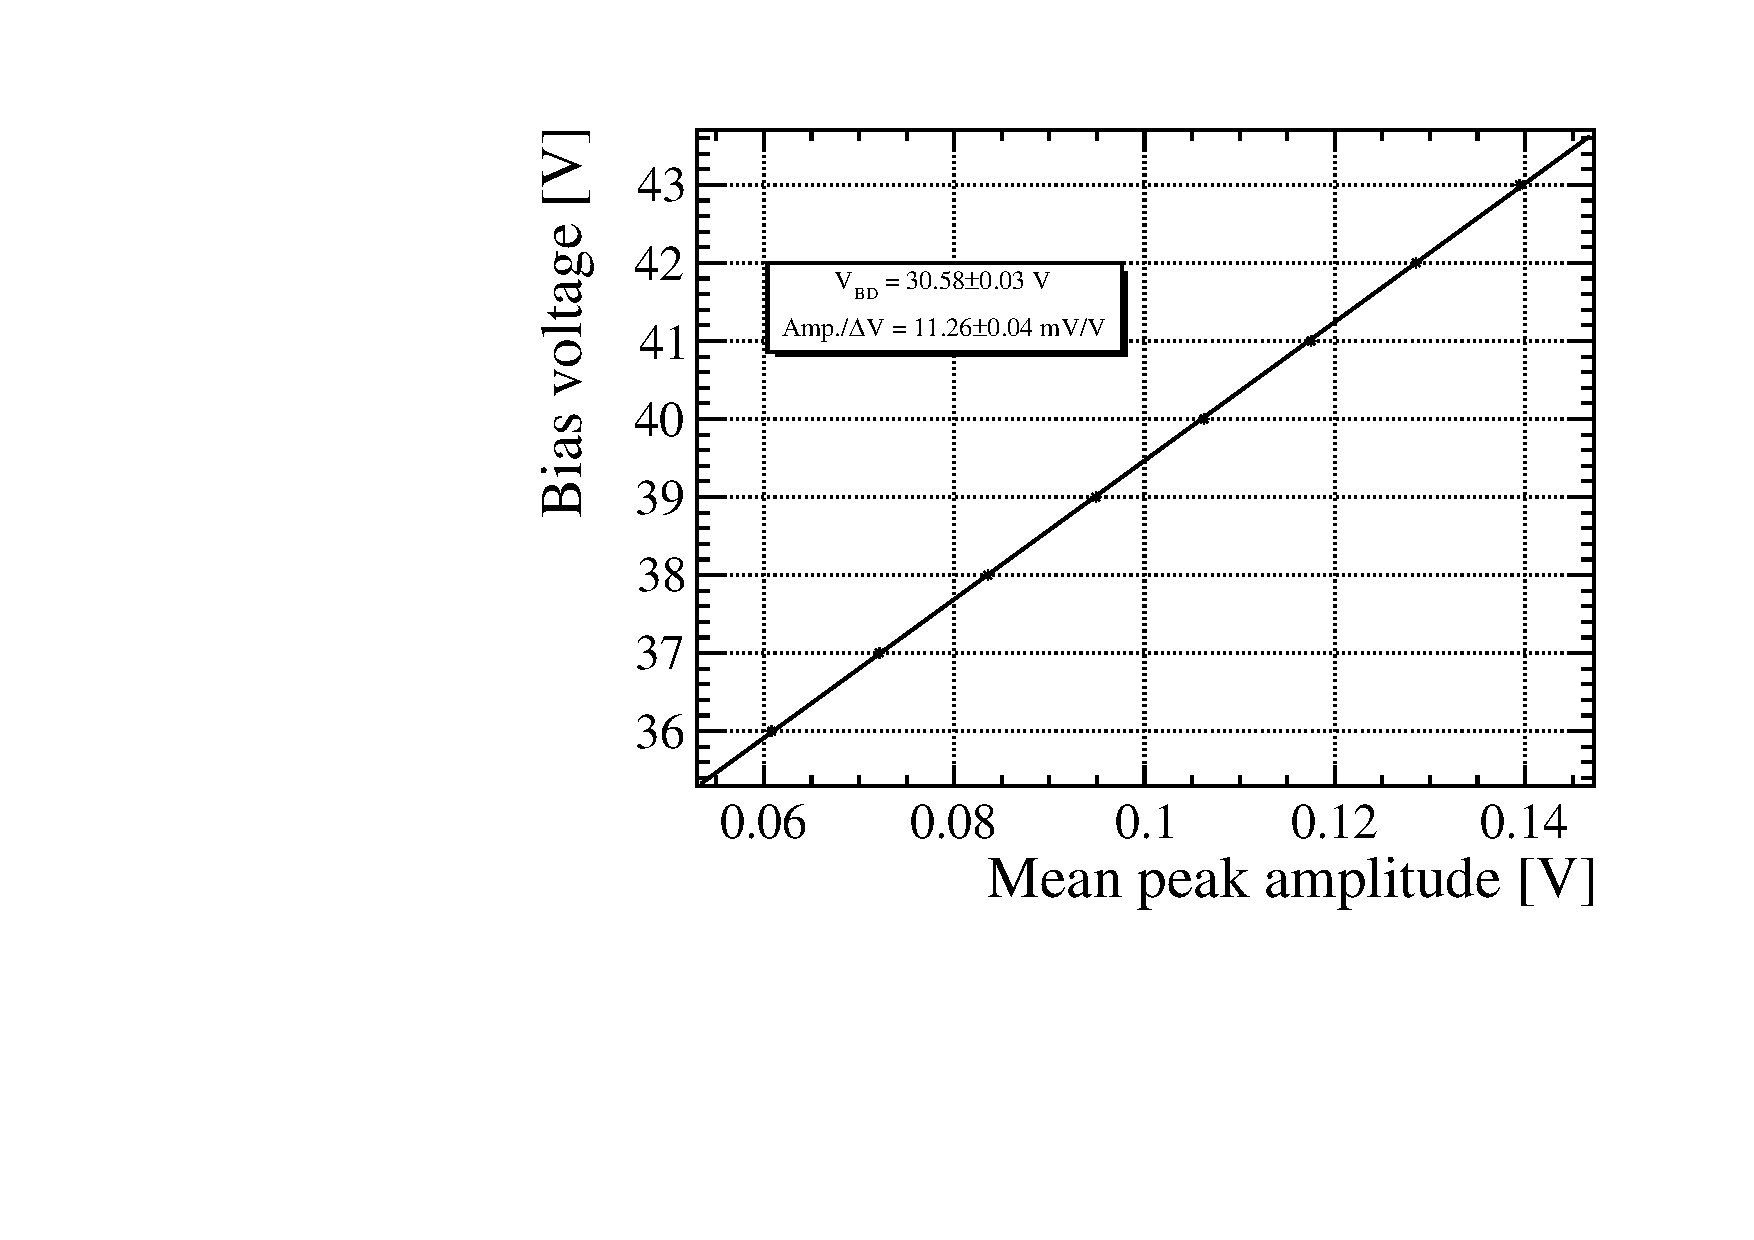
\includegraphics[width=1\linewidth]{gfx/plots/WA/16/Breakdown_voltage86.pdf}
    \caption{\SI{16}{\micro m} channel $86$.}   
  \end{subfigure}
  \hfill
  \begin{subfigure}{0.48\textwidth}
    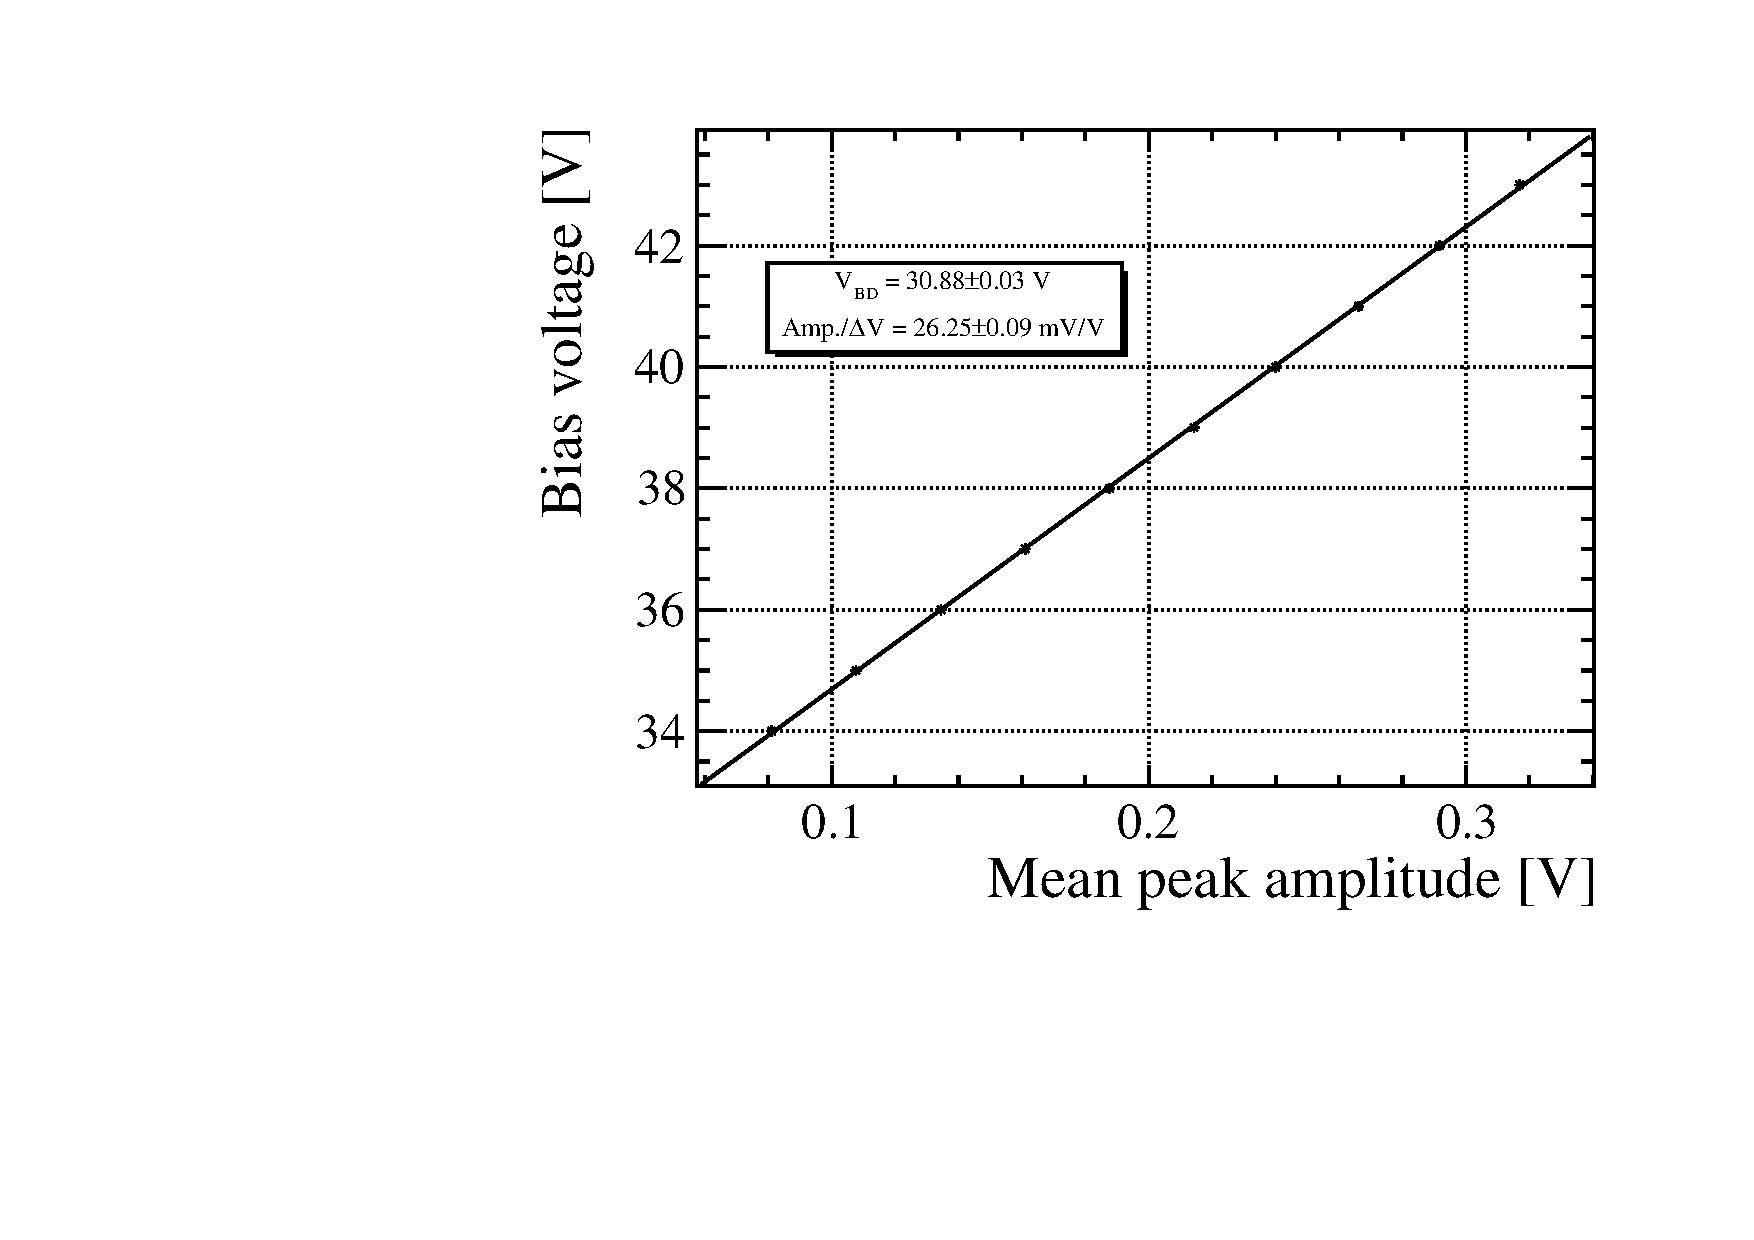
\includegraphics[width=1\linewidth]{gfx/plots/WA/31/Breakdown_voltage6.pdf}
    \caption{\SI{31}{\micro m} channel $6$.}  
  \end{subfigure}
  \hfill  
  \begin{subfigure}{0.48\textwidth}
    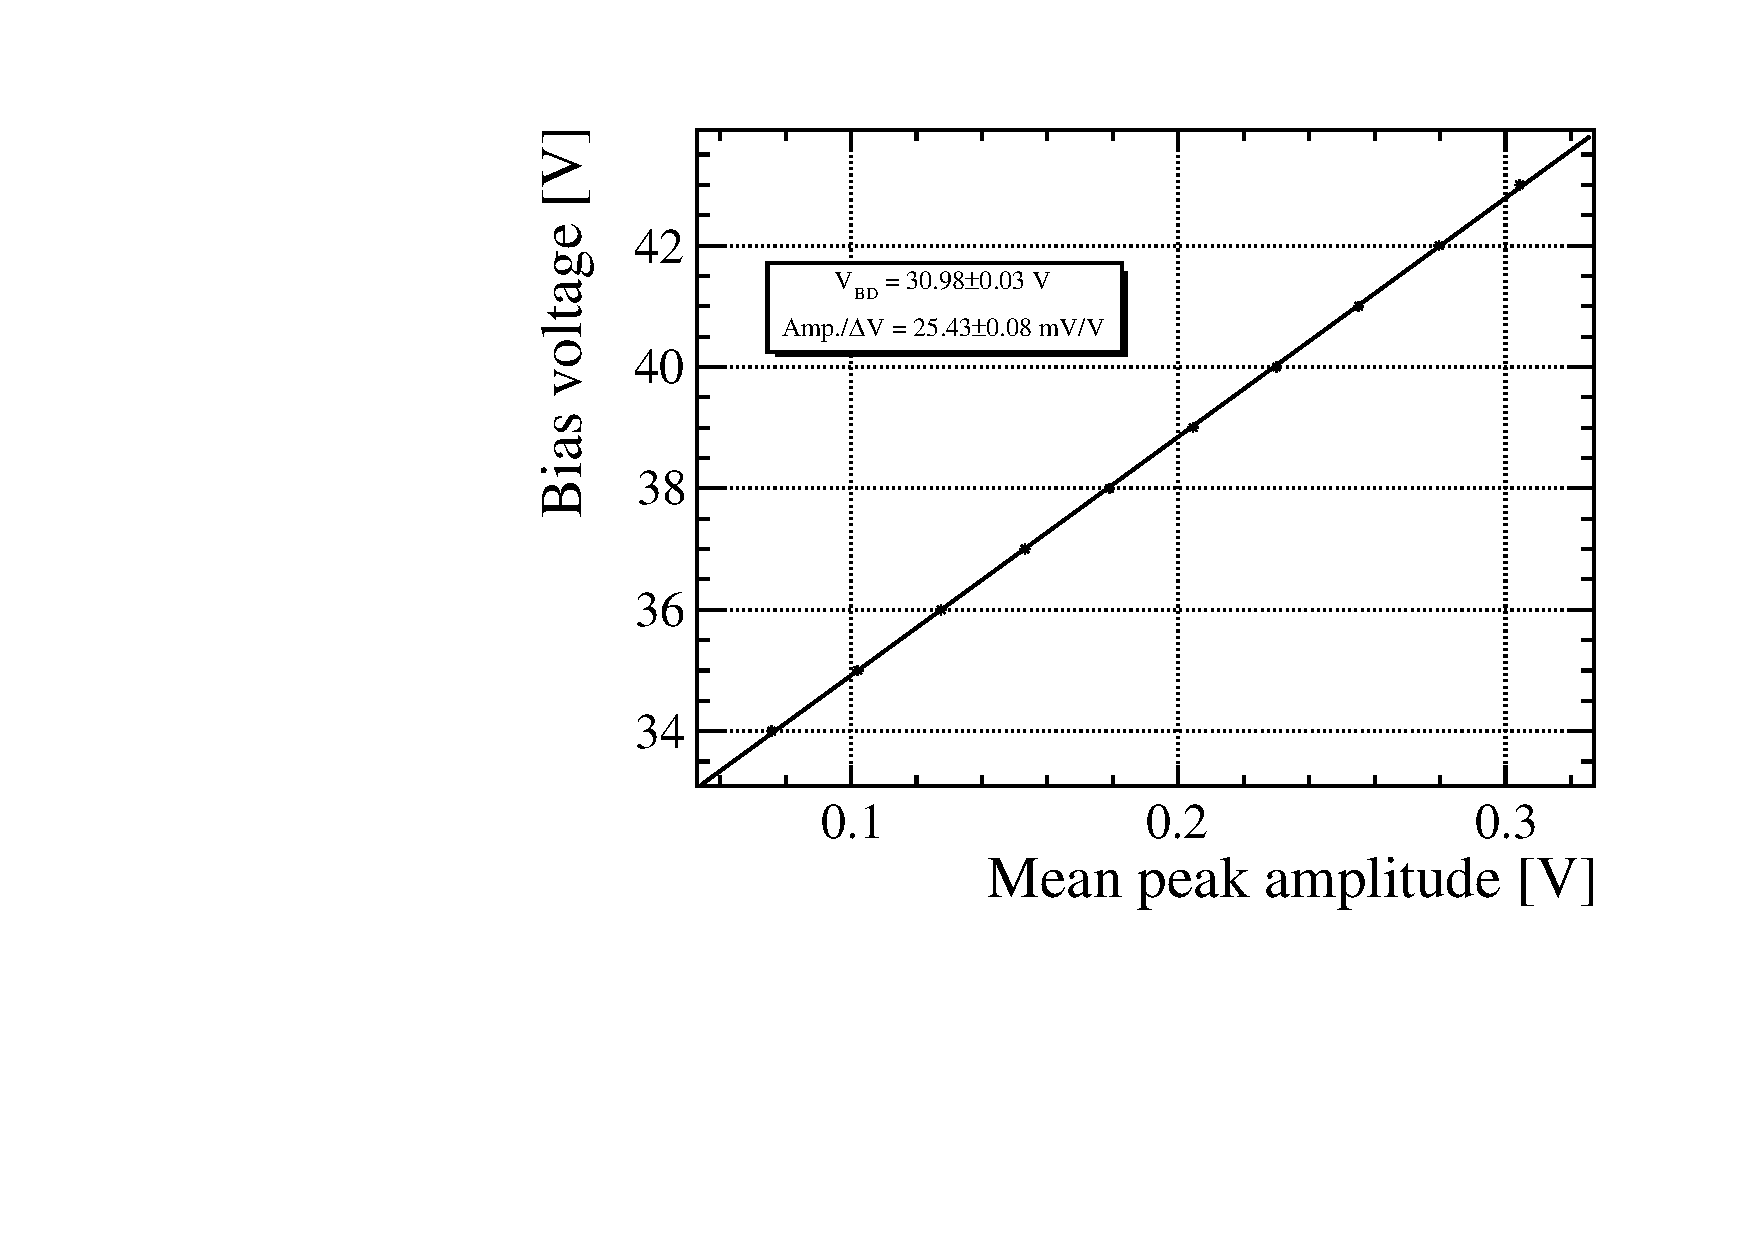
\includegraphics[width=1\linewidth]{gfx/plots/WA/31/Breakdown_voltage36.pdf}
    \caption{\SI{31}{\micro m} channel $36$.}
  \end{subfigure}
  \hfill 
  \begin{subfigure}{0.48\textwidth}
    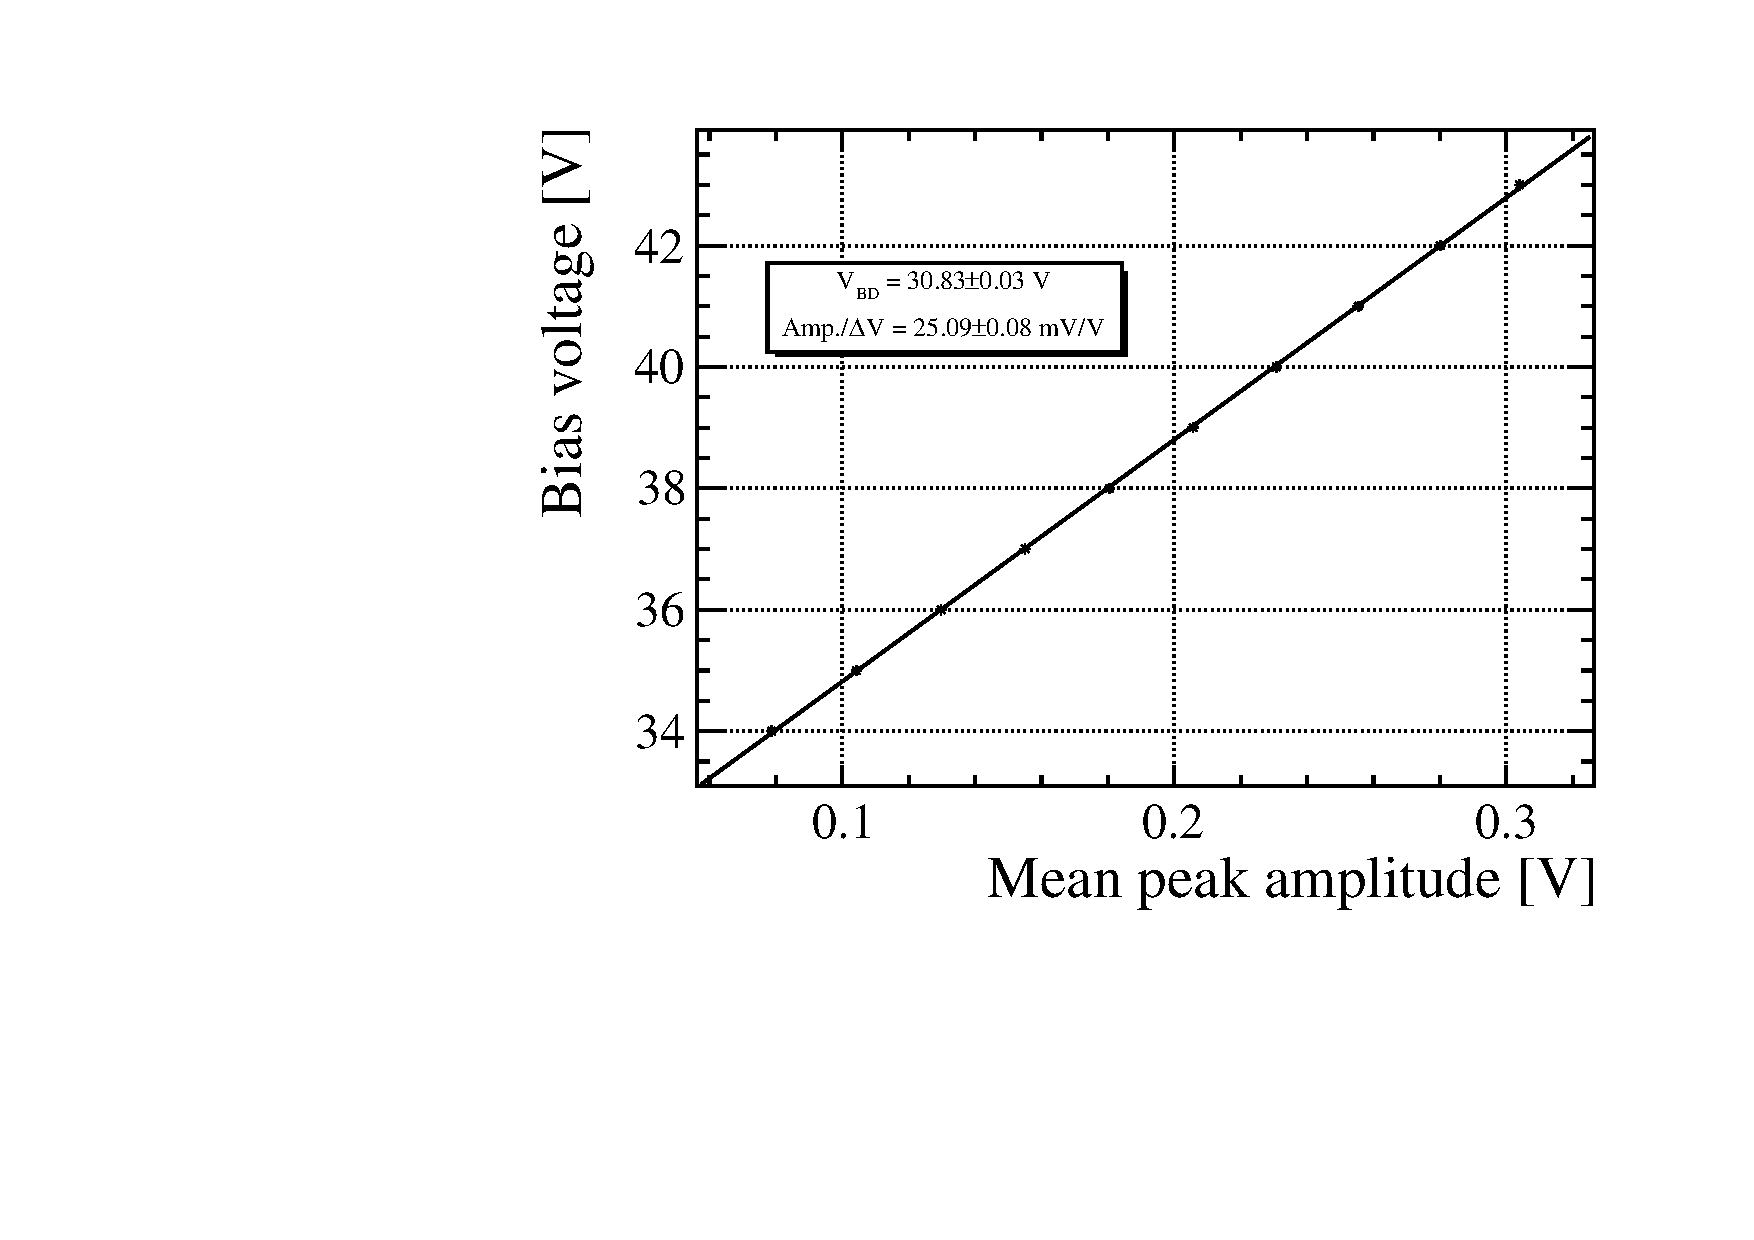
\includegraphics[width=1\linewidth]{gfx/plots/WA/31/Breakdown_voltage86.pdf}
    \caption{\SI{31}{\micro m} channel $86$.}
  \end{subfigure}
  \caption{}
  \label{}
\end{figure}

\begin{figure}
    \centering
  \begin{subfigure}{0.48\textwidth}
    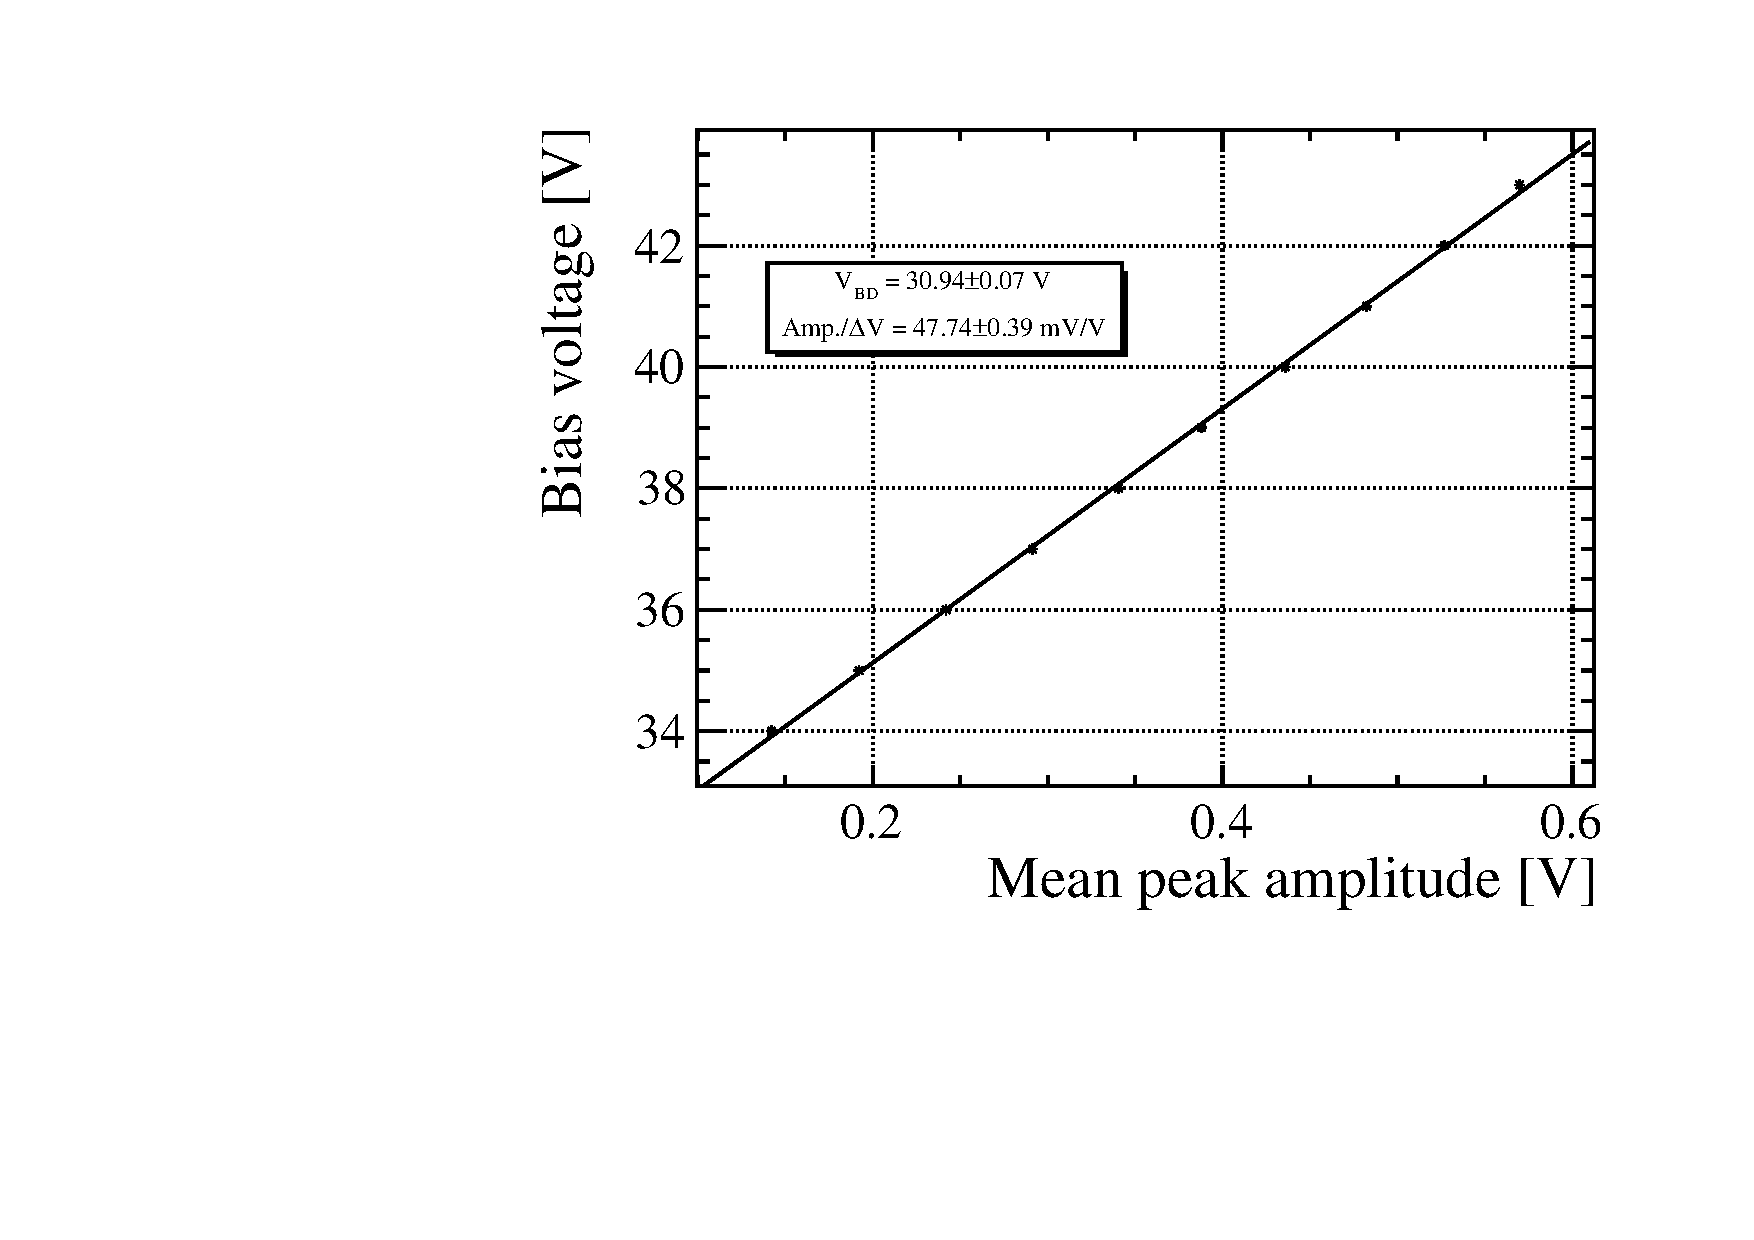
\includegraphics[width=1\linewidth]{gfx/plots/WA/42/Breakdown_voltage22.pdf}
    \caption{\SI{42}{\micro m} channel $22$.}
  \end{subfigure}
  \hfill
  \begin{subfigure}{0.48\textwidth}
    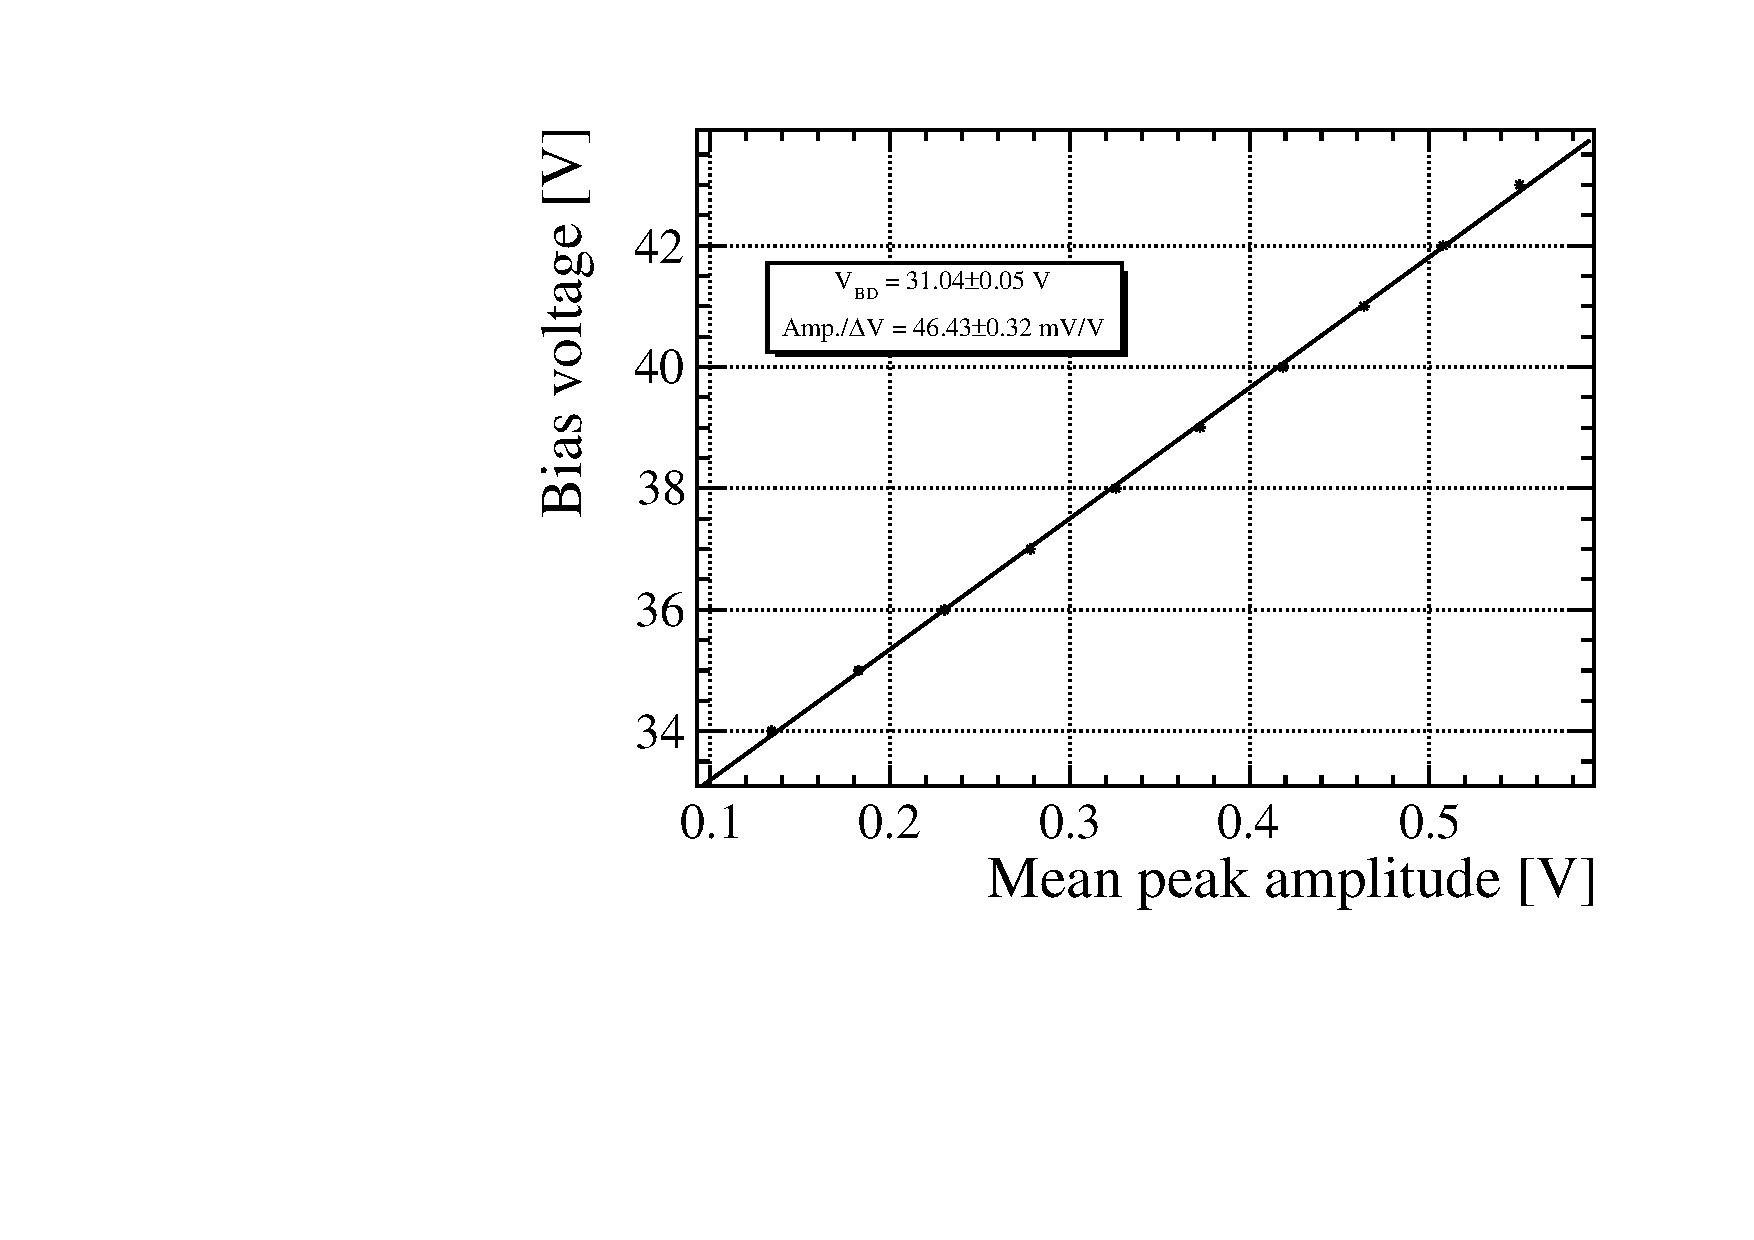
\includegraphics[width=1\linewidth]{gfx/plots/WA/42/Breakdown_voltage102.pdf}
    \caption{\SI{42}{\micro m} channel $102$.}
  \end{subfigure}
  \hfill
  \begin{subfigure}{0.48\textwidth}
    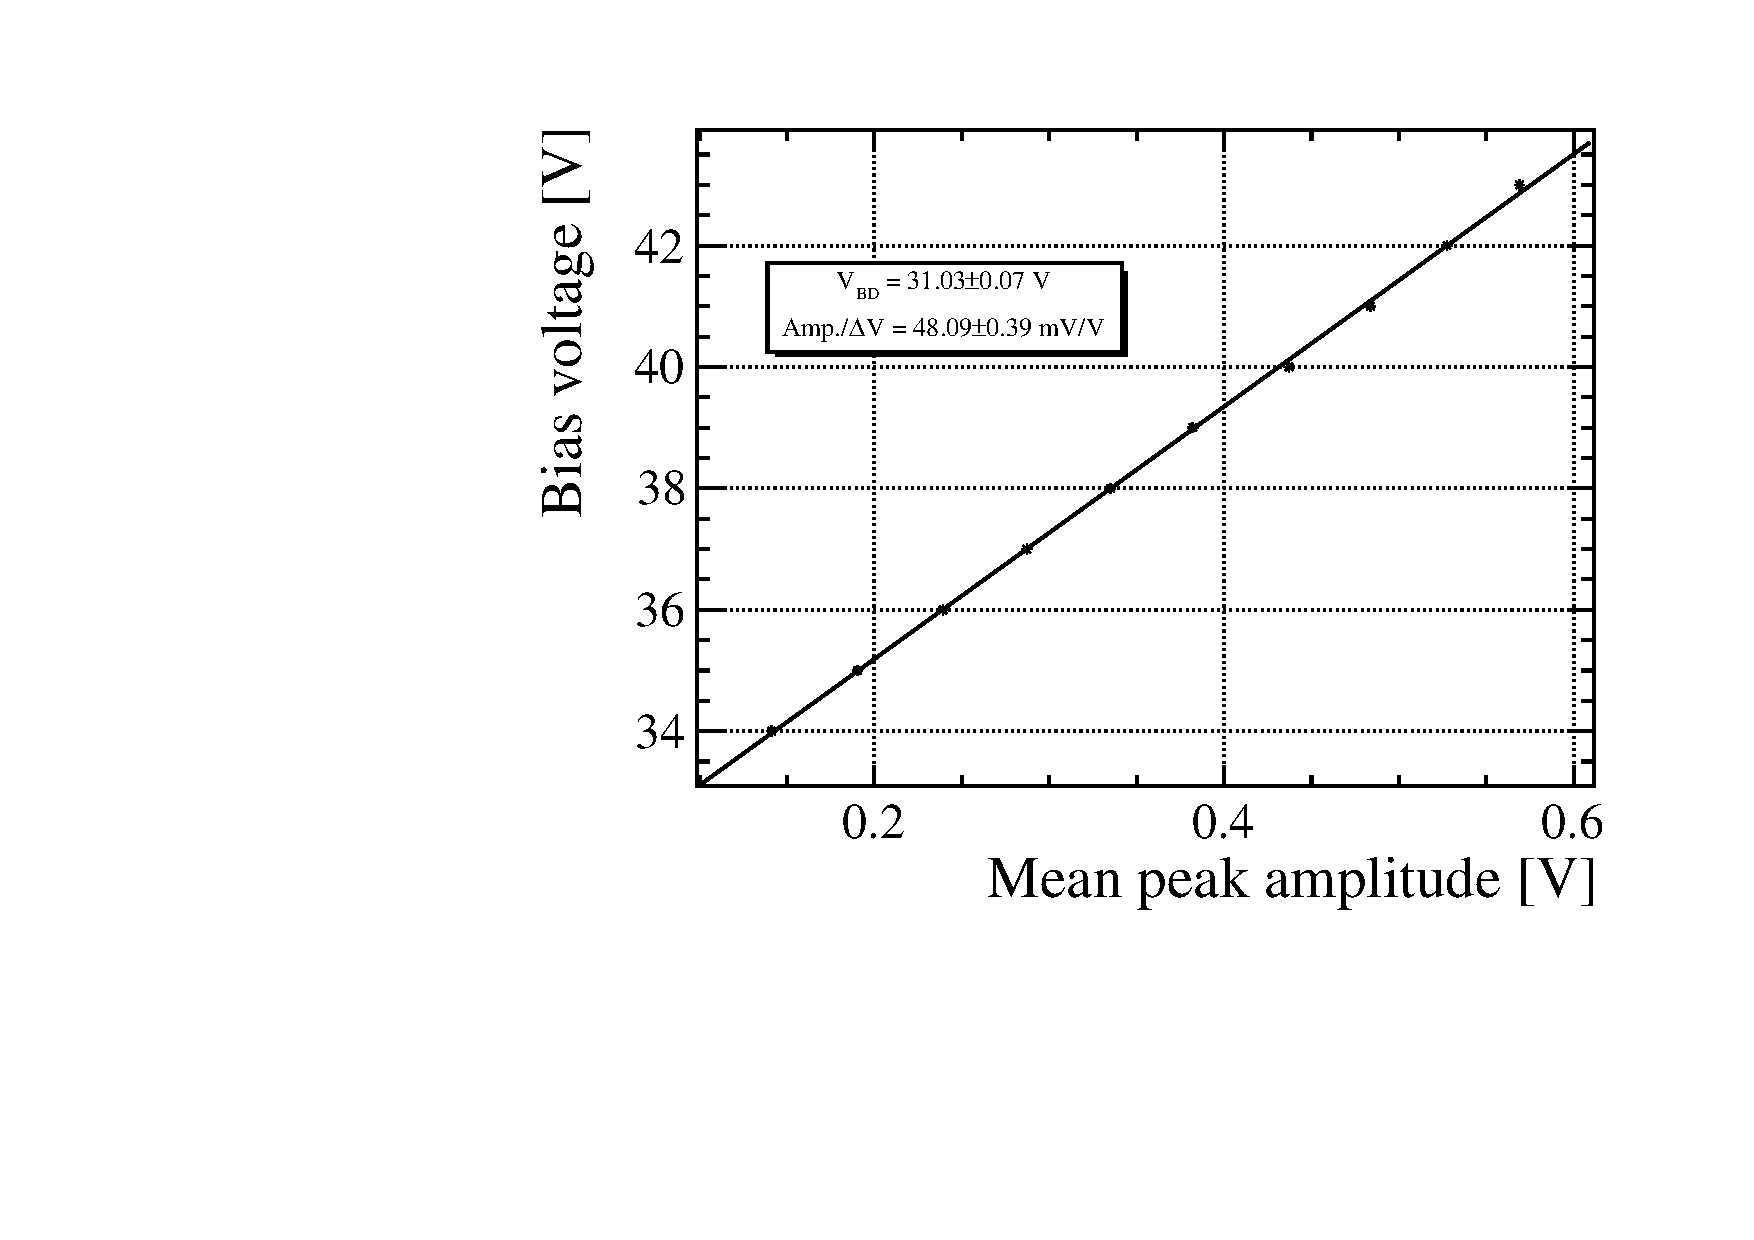
\includegraphics[width=1\linewidth]{gfx/plots/WA/42/Breakdown_voltage54.pdf}
    \caption{\SI{42}{\micro m} channel $54$.}
  \end{subfigure}
  \hfill
  \begin{subfigure}{0.48\textwidth}
    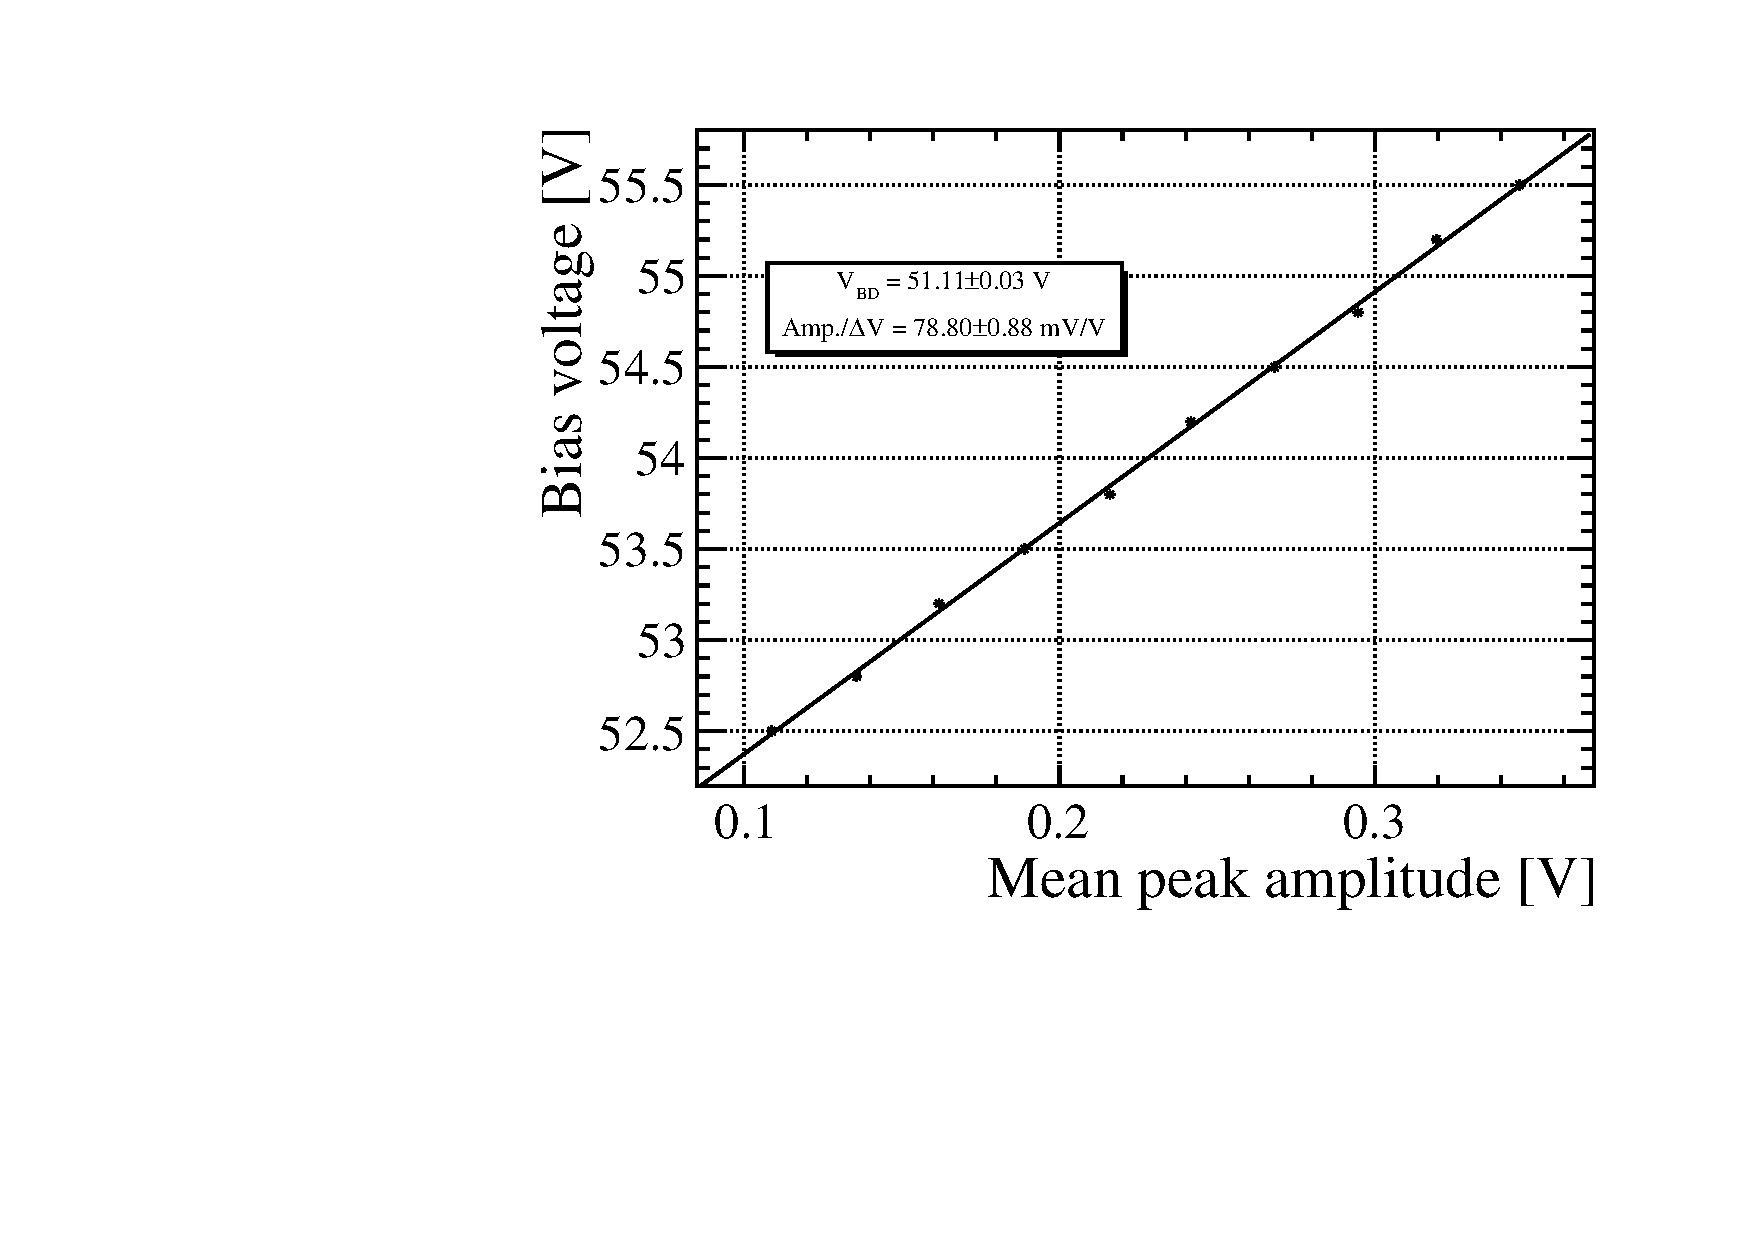
\includegraphics[width=1\linewidth]{gfx/plots/WA/H2017/Breakdown_voltage54.pdf}
    \caption{H2017 channel $54$.}
  \end{subfigure}
  \hfill
  \begin{subfigure}{0.48\textwidth}
    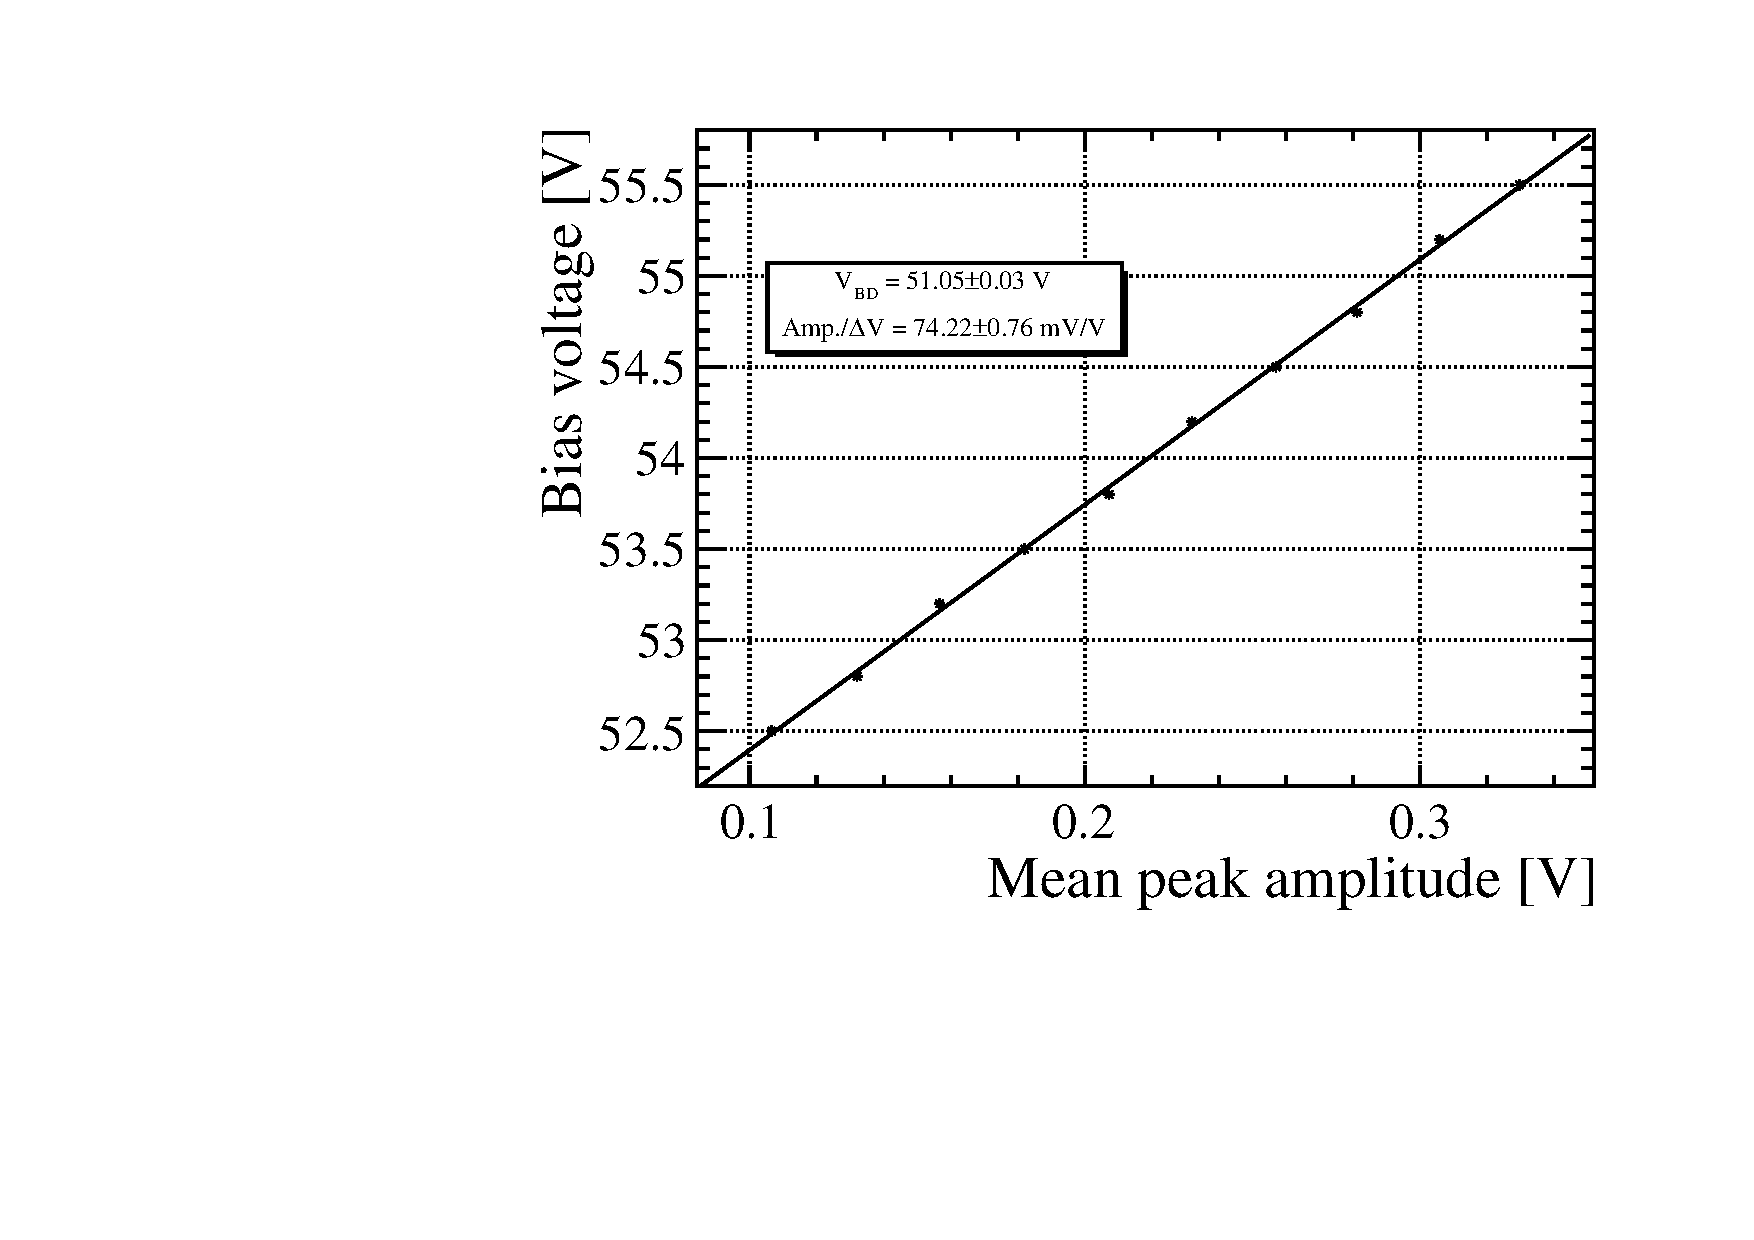
\includegraphics[width=1\linewidth]{gfx/plots/WA/H2017/Breakdown_voltage86.pdf}
    \caption{H2017 channel $86$.}
  \end{subfigure}
\caption{}
\label{appendix:fig:Vbd fits}
\end{figure}


\section{Correlated noise}

\begin{figure}[hbtp]
    \centering
    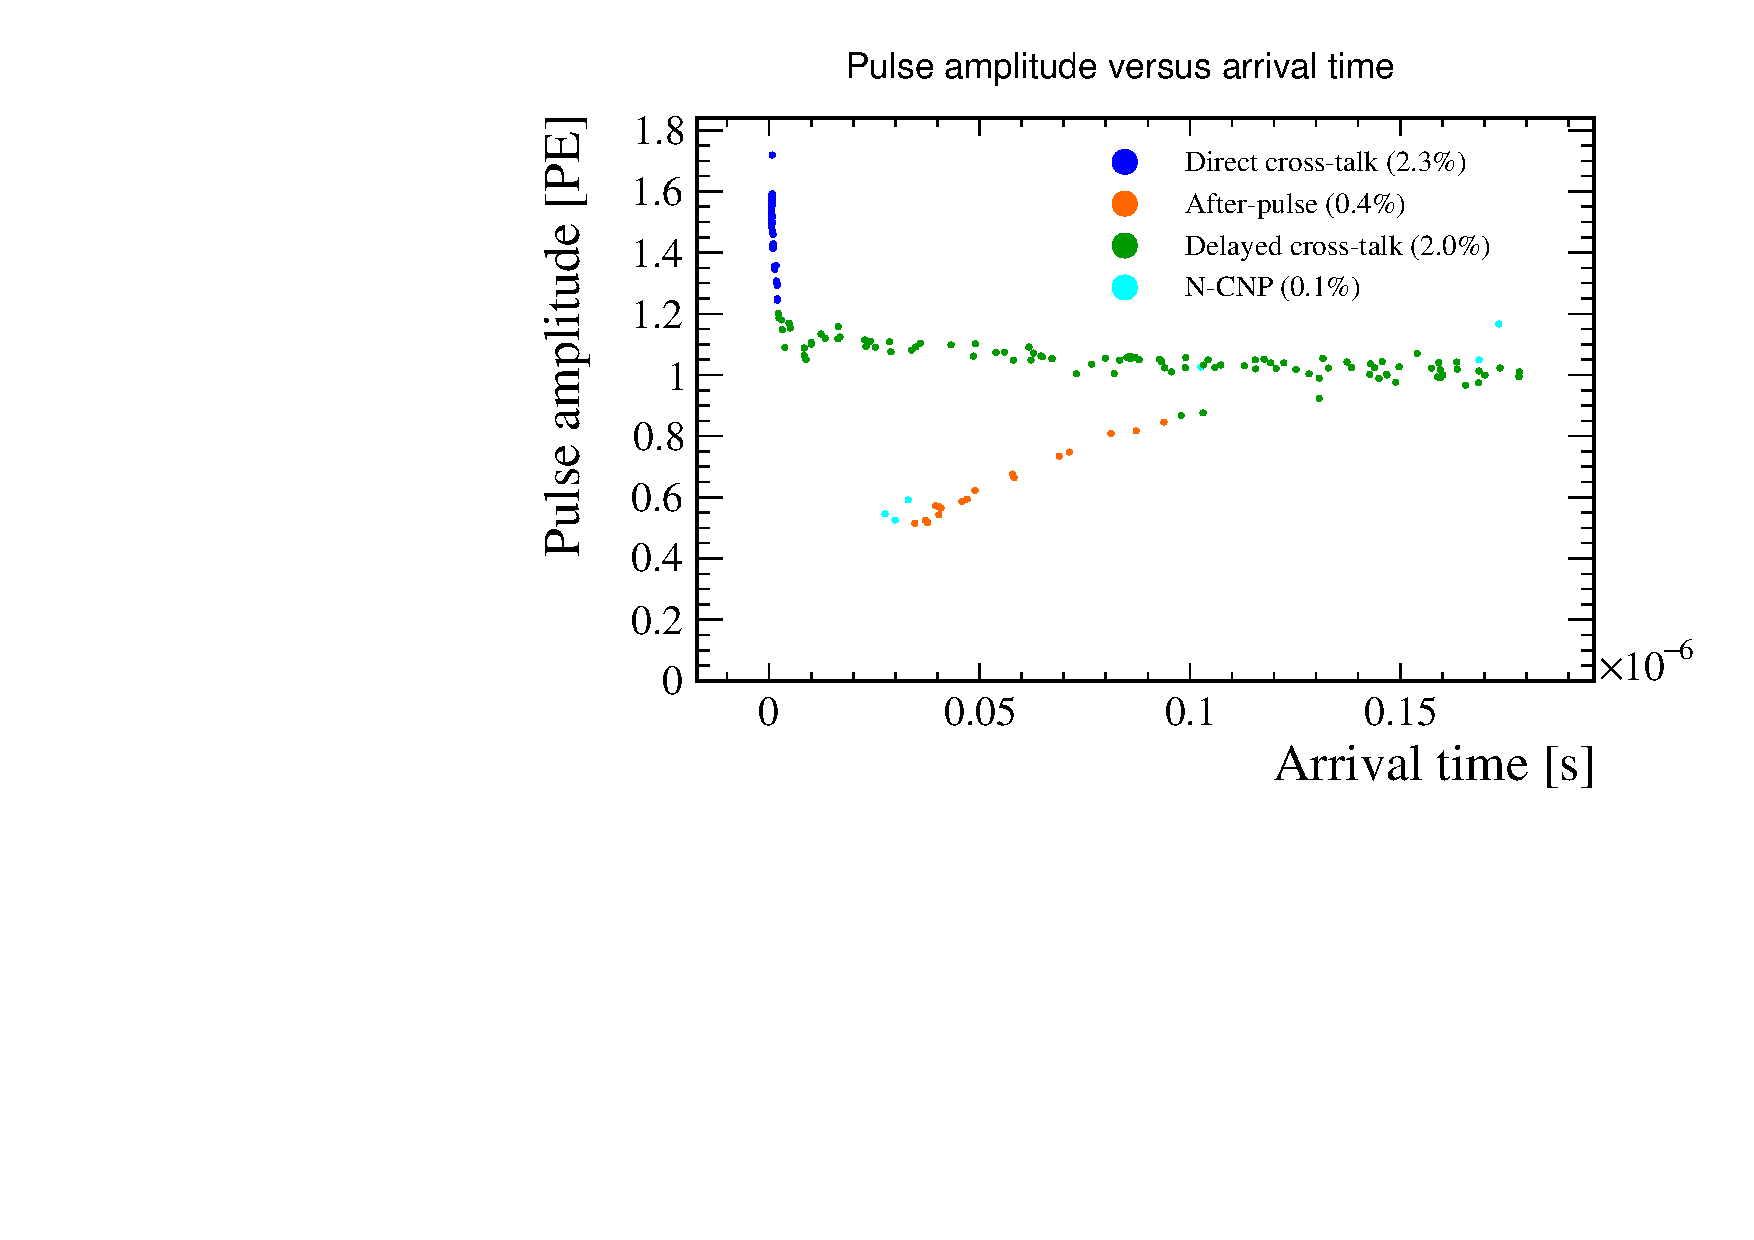
\includegraphics[width=1\textwidth]{gfx/plots/WA/42/peakamptime.pdf}
    \caption{FBK \SI{42}{\micro m} detector.}   
    \label{fig:peakamptime 42}
\end{figure}

%\section{Gain}

